\documentclass{article}

\usepackage{graphicx}
\usepackage{tikz}
\usepackage{tikzsymbols}
\usetikzlibrary{calc,patterns,shapes.geometric}
\pagestyle{empty}
\usepackage[margin=0pt]{geometry}
\geometry{papersize={14in,12in}}

\def\centerarc[#1](#2)(#3:#4:#5){\draw[#1] ($(#2)+({#5*cos(#3)},{#5*sin(#3)})$) arc (#3:#4:#5);}

\begin{document}
	\begin{figure}
		\centering
		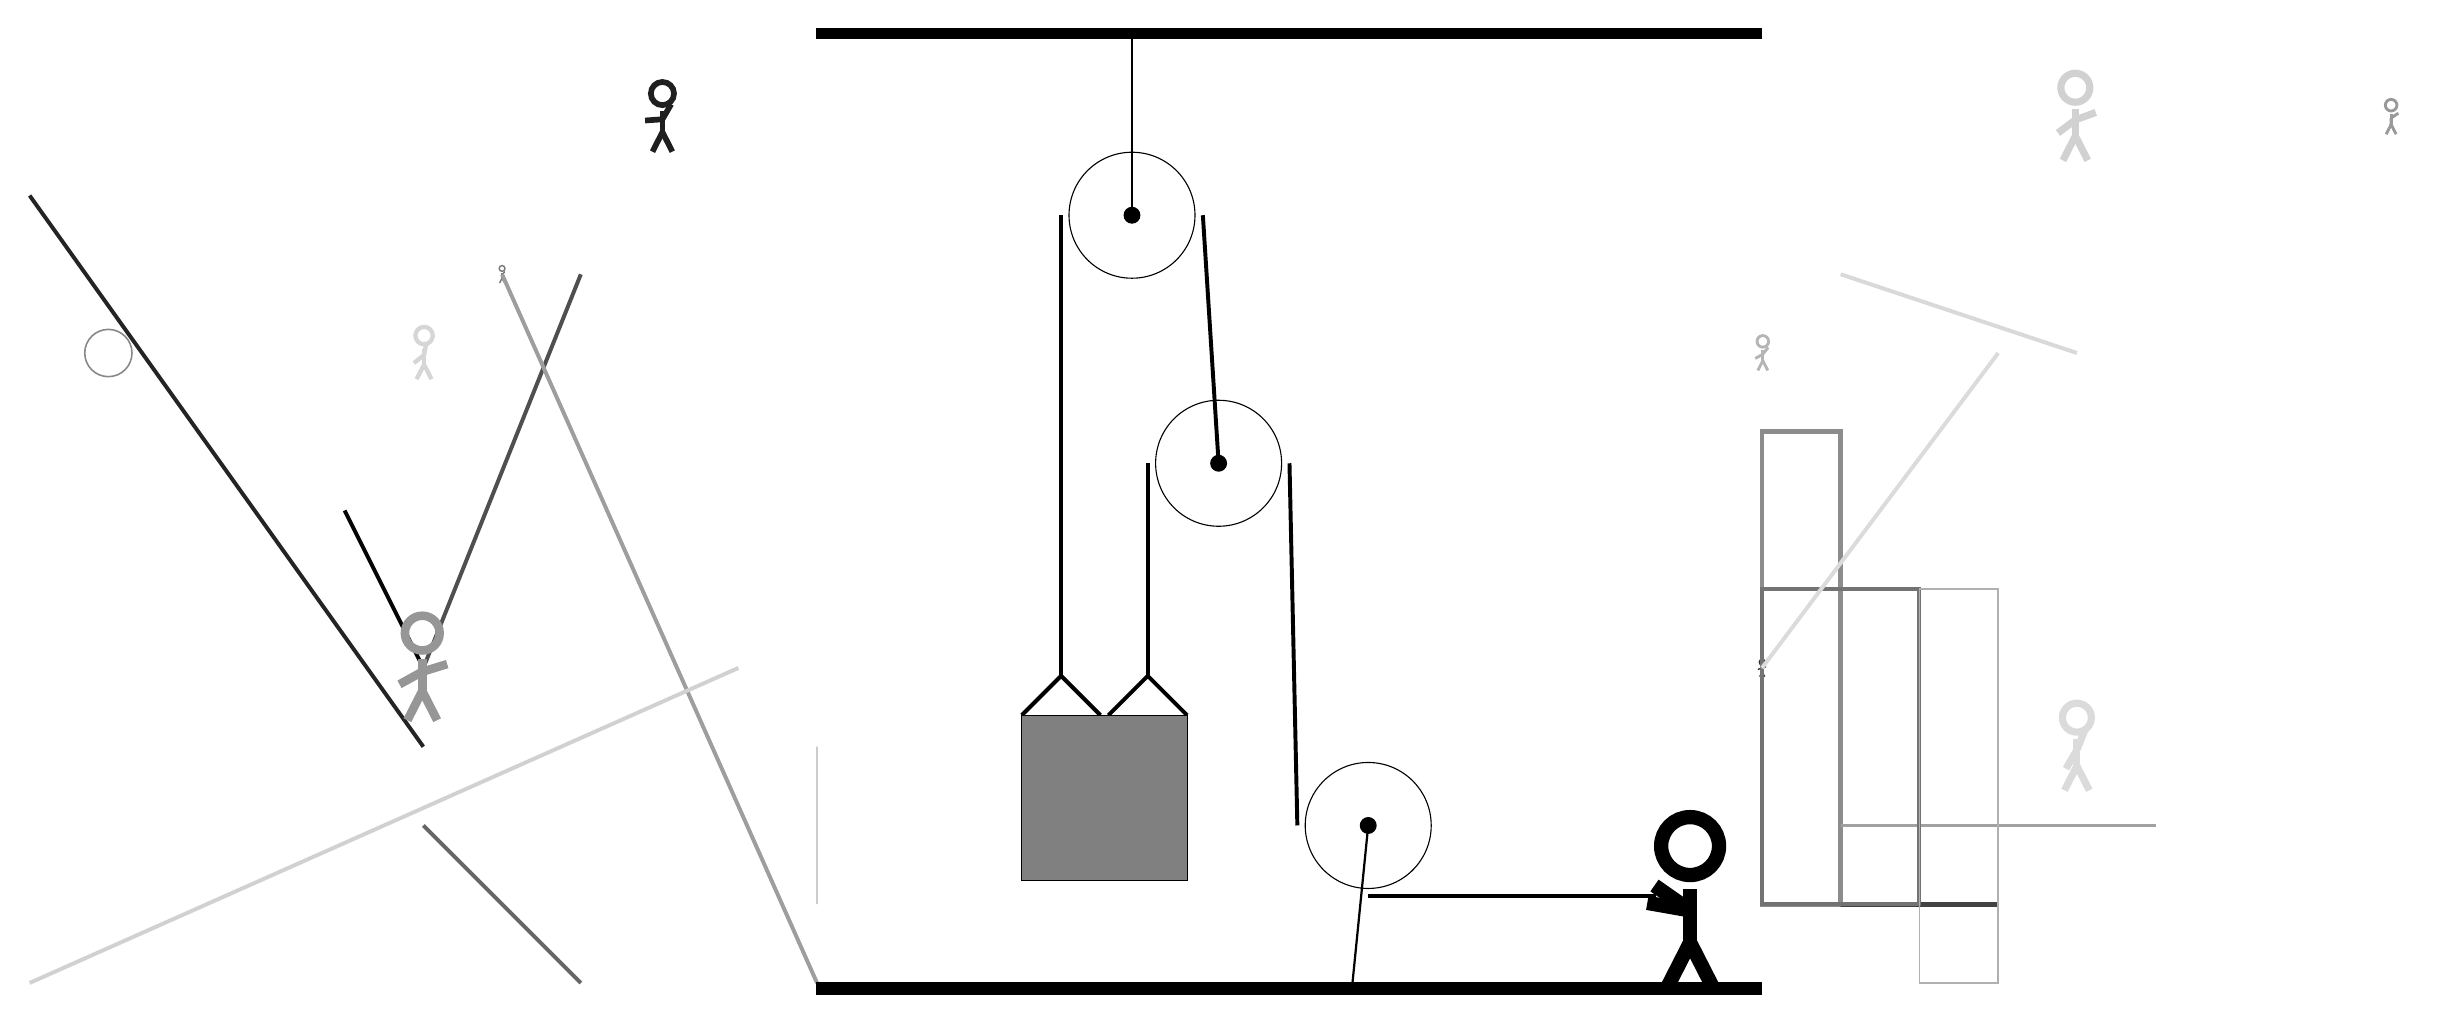
\begin{tikzpicture}
			%%%%% START %%%%%
			
			\draw[fill=black] (-2, 9) rectangle (10, 9.125);
			
			\draw (2, 6.75) circle (0.8);
			\draw[fill=black] (2, 6.75) circle (0.1);
			\draw[thick] (2, 6.75) -- (2, 9);
			
			\draw (3.1, 3.6) circle (0.8);
			\draw[fill=black] (3.1, 3.6) circle (0.1);
			
			\draw (5, -1) circle (0.8);
			\draw[fill=black] (5, -1) circle (0.1);
			\draw[thick] (5, -1) -- (4.8, -3);
			
			\draw[line width = 0.5mm]  (0.6, 0.4) -- (1.1, 0.9) -- (1.6, 0.4);
			\draw[line width = 0.5mm]  (1.7, 0.4) -- (2.2, 0.9) -- (2.7, 0.4);
			\draw[fill=black!50] (0.6, 0.4) rectangle (2.7, -1.7);
			
			\draw[line width = 0.5mm] (1.1, 6.75) -- (1.1, 0.9);
			\centerarc[line width = 0.5mm](2, 6.75)(0:180:0.9);
			\draw[line width = 0.5mm] (2.9, 6.75) -- (3.1, 3.6);
			\draw[line width = 0.5mm] (2.2, 3.6) -- (2.2, 0.9);
			\centerarc[line width = 0.5mm](3.1, 3.6)(0:180:0.9);
			\draw[line width = 0.5mm] (4.0, 3.6) -- (4.1, -1);
			\centerarc[line width = 0.5mm](5, -1)(180:270:0.9);
			\draw[line width = 0.5mm] (5, -1.9) -- (8.65, -1.9);
			
			\node at (9, -2) {\Strichmaxerl[10][-35][170]};
			
			\draw[line width=0.6mm, color=black!45] (10, -2) rectangle (11, 4);
			
			\draw[line width=0.5mm, color=black!69](-7, 1) -- (-5, 6);
			\node[line width=0.2mm, color=black!40] at (18, 8) {\Strichmaxerl[2][88][34]};
			\draw[line width=0.5mm, color=black!37](15, -1) -- (11, -1);
			\node[line width=0.2mm, color=black!88] at (-4, 8) {\Strichmaxerl[4][4][60]};
			\draw[line width=0.6mm, color=black!74] (11, -2) rectangle (13, -2);
			
			\draw[line width=0.5mm, color=black!61](12, 1) -- (12, 2);
			\node[line width=0.3mm, color=black!81] at (10, 1) {\Strichmaxerl[1][7][29]};
			\node[line width=0.3mm, color=black!52] at (-6, 6) {\Strichmaxerl[1][87][50]};
			
			\draw[line width=0.2mm, color=black!90] (-4, 0) rectangle (-4, 0);
			
			\draw[line width=0.5mm, color=black!38](-2, -3) -- (-6, 6);
			\draw[line width=0.5mm, color=black!86](-7, 0) -- (-12, 7);
			\draw[line width=0.3mm, color=black!20] (-2, 0) rectangle (-2, -2);
			
			\draw[line width=0.5mm, color=black!15](11, 6) -- (14, 5);
			\draw [line width=0.2mm, color=black!47](-11, 5) circle (0.3);
			\draw[line width=0.5mm, color=black!98](-7, 1) -- (-8, 3);
			
			\draw[line width=0.5mm, color=black!55] (10, -2) rectangle (12, 2);
			
			\draw[line width=0.5mm, color=black!18](-3, 1) -- (-12, -3);
			\node[line width=0.5mm, color=black!41] at (-7, 1) {\Strichmaxerl[6][29][17]};
			\draw[line width=0.5mm, color=black!60](-7, -1) -- (-5, -3);
			\node[line width=0.3mm, color=black!18] at (14, 8) {\Strichmaxerl[5][37][20]};
			\node[line width=0.6mm, color=black!29] at (10, 5) {\Strichmaxerl[2][29][52]};
			
			\node[line width=0.2mm, color=black!16] at (-7, 5) {\Strichmaxerl[3][39][79]};
			\draw[line width=0.5mm, color=black!14](10, 1) -- (13, 5);
			\node[line width=0.7mm, color=black!14] at (14, 0) {\Strichmaxerl[5][60][68]};
			\draw[line width=0.2mm, color=black!31] (12, 2) rectangle (13, -3);
			
			\draw[fill=black] (-2, -3) rectangle (10, -3.15);
			
			%%%%% END %%%%%
		\end{tikzpicture}
	\end{figure}	
\end{document}